%%% Preamble
\documentclass{report}

\usepackage[utf8]{inputenc}
\usepackage[T1]{fontenc}
\usepackage{fourier}
\usepackage[french]{babel}
\usepackage[protrusion=true,expansion=true]{microtype}	
\usepackage{amsmath,amsfonts,amsthm} % Math packages
\usepackage[pdftex]{graphicx}	
\usepackage{url}
\usepackage{pdfpages}
\usepackage{todonotes}
\usepackage[a4paper, body={16cm,26cm}]{geometry}
\usepackage{float}
\usepackage{framed}
\usepackage[toc,page]{appendix} 
\usepackage{multicol}
\usepackage{colortbl}
\usepackage{epstopdf}
\usepackage{adjustbox}

%%% Custom sectioning
\usepackage{sectsty}
\allsectionsfont{  \normalfont\scshape}
%\allsectionsfont{\centering \normalfont\scshape}

%%% Custom headers/footers (fancyhdr package)
\usepackage{fancyhdr}
\pagestyle{fancyplain}
\fancyhead{}								% No page header
\fancyfoot[L]{}							% Empty 
\fancyfoot[C]{}							% Empty
\fancyfoot[R]{\thepage}					% Pagenumbering
\renewcommand{\headrulewidth}{0pt}		% Remove header underlines
\renewcommand{\footrulewidth}{0pt}		% Remove footer underlines
\setlength{\headheight}{13.6pt}


%%% Equation and float numbering
\numberwithin{equation}{section}		% Equationnumbering: section.eq#
\numberwithin{figure}{section}		% Figurenumbering: section.fig#
\numberwithin{table}{section}		% Tablenumbering: section.tab#


%%% Define new commands
\newcommand{\horrule}[1]{\rule{\linewidth}{#1}} 	% Horizontal rule
\renewcommand{\bf}[1]{\textbf{#1}}
\renewcommand{\it}[1]{\textit{#1}}
\newcommand{\bfit}[1]{\textbf{\textit{#1}}}
\renewcommand{\sc}[1]{\textsc{#1}}

\newcommand{\Todo}[1]{\todo[inline]{#1}}
\renewcommand{\thesection}{\thepart .\arabic{section}}

\usepackage{tocloft}
\cftsetindents{chapter}{0em}{1em}
\cftsetindents{section}{1.5em}{2.5em}
\makeatletter
\def\l@figure{\@dottedtocline{1}{1.5em}{4em}}
\makeatother

\usepackage{bookmark}
%\usepackage[hidelinks]{hyperref}
\usepackage{cases}
\usepackage{color}
\usepackage{xcolor}
\usepackage{relsize}
\usepackage{caption}
\colorlet{shadecolor}{black!10}

\delimitershortfall-1sp
\newcommand\abs[1]{\left|#1\right|}


\usepackage{tikz, pgfplots}


%}}}
%{{{ --- pgfplots ---------------------

%{{{ Colors

% TolColors from http://www.r-bloggers.com/the-paul-tol-21-color-salute/
\definecolor{TolColor1}{HTML}{332288}   % dark purple
\definecolor{TolColor2}{HTML}{6699CC}   % dark blue
\definecolor{TolColor3}{HTML}{88CCEE}   % light blue
\definecolor{TolColor4}{HTML}{44AA99}   % light green
\definecolor{TolColor5}{HTML}{117733}   % dark green
\definecolor{TolColor6}{HTML}{999933}   % dark brown
\definecolor{TolColor7}{HTML}{DDCC77}   % light brown
\definecolor{TolColor8}{HTML}{661100}   % dark red
\definecolor{TolColor9}{HTML}{CC6677}   % light red
\definecolor{TolColor10}{HTML}{AA4466}  % light pink
\definecolor{TolColor11}{HTML}{882255}  % dark pink
\definecolor{TolColor12}{HTML}{AA4499}  % light purple

%}}}
%{{{ Color cycles

\pgfplotscreateplotcyclelist{mbarplot cycle}{%
  {draw=TolColor2, fill=TolColor2!70},
  {draw=TolColor7, fill=TolColor7!70},
  {draw=TolColor4, fill=TolColor4!70},
  {draw=TolColor11, fill=TolColor11!70},
  {draw=TolColor1, fill=TolColor1!70},
  {draw=TolColor8, fill=TolColor8!70},
  {draw=TolColor6, fill=TolColor6!70},
  {draw=TolColor9, fill=TolColor9!70},
  {draw=TolColor10, fill=TolColor10!70},
  {draw=TolColor12, fill=TolColor12!70},
  {draw=TolColor3, fill=TolColor3!70},
  {draw=TolColor5, fill=TolColor5!70},
}

\pgfplotscreateplotcyclelist{mlineplot cycle}{%
  {TolColor2, mark=*, mark size=1.5pt},
  {TolColor7, mark=square*, mark size=1.3pt},
  {TolColor4, mark=triangle*, mark size=1.5pt},
  {TolColor6, mark=diamond*, mark size=1.5pt},
}


\pgfplotsset{
  compat=1.9,
  mbaseplot/.style={
    legend style={
      draw=none,
      fill=none,
      cells={anchor=west},
    },
    x tick label style={
      font=\footnotesize
    },
    y tick label style={
      font=\footnotesize
    },
    legend style={
      font=\footnotesize
    },
    major grid style={
      dotted,
    },
    axis x line*=bottom,
  },
  mlineplot/.style={
    mbaseplot,
    xmajorgrids=true,
    ymajorgrids=true,
    major grid style={dotted},
    axis x line=bottom,
    axis y line=left,
    legend style={
      cells={anchor=west},
      draw=none
    },
    cycle list name=mlineplot cycle,
  },
  mbarplot base/.style={
    mbaseplot,
    bar width=6pt,
    axis y line*=none,
  },
  mbarplot/.style={
    mbarplot base,
    ybar,
    xmajorgrids=false,
    ymajorgrids=true,
    area legend,
    legend image code/.code={%
      \draw[#1] (0cm,-0.1cm) rectangle (0.15cm,0.1cm);
    },
    cycle list name=mbarplot cycle,
  },
  horizontal mbarplot/.style={
    mbarplot base,
    xmajorgrids=true,
    ymajorgrids=false,
    xbar stacked,
    area legend,
    legend image code/.code={%
      \draw[#1] (0cm,-0.1cm) rectangle (0.15cm,0.1cm);
    },
    cycle list name=mbarplot cycle,
  },
  disable thousands separator/.style={
    /pgf/number format/.cd,
      1000 sep={}
  },
}


%%  ========   IMPORTANT ========
%% Spécifier ici les variables pour le document
\newcommand{\mainTitle}{\'Etude préalable - SPIE}
\newcommand{\secondTitle}{Document de suivi}
\newcommand{\documentRef}{TB/4401/1}

%%% Begin document
\begin{document}
%----------------------------------------------------------------------------------------
%	PACKAGES
%----------------------------------------------------------------------------------------

\documentclass[12pt]{article}
\usepackage[a4paper]{geometry}
\geometry{verbose,tmargin=1in,bmargin=0in,lmargin=1in,rmargin=1in}
\usepackage[utf8]{inputenc}
\usepackage[francais]{babel}
\usepackage[T1]{fontenc}

\usepackage{graphicx}
\begin{document}

\begin{titlepage}

\newcommand{\HRule}{\rule{\linewidth}{0.5mm}} % horizontal lines

\center % Center everything
 
%----------------------------------------------------------------------------------------
%	HEADING SECTIONS
%----------------------------------------------------------------------------------------

\vspace*{1cm}

\textsc{\LARGE INSA de LYON}\\[1.5cm] 
\textsc{\Large D\'epartement Informatique}\\[0.5cm] 
\textsc{\large Projet Longue Durée}\\[0.5cm] % 

%----------------------------------------------------------------------------------------
%	TITLE SECTION
%----------------------------------------------------------------------------------------

\HRule \\[0.4cm]
{ \huge \bfseries Compte Rendu}\\[0.1cm]
{\large \bfseries - Gestion des contacts commerciaux d'une banque -} 
\HRule \\[1.5cm]
 
%----------------------------------------------------------------------------------------
%	DATE SECTION
%----------------------------------------------------------------------------------------

{\large \today}\\[2cm] % 
 
%----------------------------------------------------------------------------------------
%	AUTHOR SECTION
%----------------------------------------------------------------------------------------

\begin{minipage}{0.4\textwidth}
\begin{center} \large
\emph{Auteurs} \\
Lisa \textsc{Courant} \\
Estelle \textsc{Lepeigneux} \\
Pierre \textsc{Jarsaillon} \\
Hugues \textsc{Verlin} \\
\end{center}
\end{minipage}
~
\begin{minipage}{0.4\textwidth}
\begin{center} \large
\emph{Chef de projet} \\
Paul \textsc{Dautry}
\end{center}
\begin{center} \large
\emph{Responsable Qualité} \\
Antoine \textsc{Chabert}
\end{center}
\end{minipage}\\[5cm]

H4401\\[2cm]

%----------------------------------------------------------------------------------------
%	LOGO SECTION
%----------------------------------------------------------------------------------------

\includegraphics[scale=0.3]{figures/logo.png}
%----------------------------------------------------------------------------------------

\vfill % Fill the rest of the page with whitespace

\end{titlepage}
\end{document}


%% Commenter les deux lignes suivantes pour le document final
%\listoftodos
\newpage

%% Table de matière / figures / tableaux
\tableofcontents
\listoffigures
\listoftables
\newpage


\part{Bilan phase d'Initialisation}

Ce bilan a été rédigé le 13 décembre 2015. Le tableau de bord associé est pésent en Annexe A.

\setcounter{section}{0}

\section{Bilan d'avancement}

Au terme de cette séance d'initialisation, l'ensemble des tâches a été réalisé dans les temps. Il n'y a donc pas, à ce stade, de glissement concernant le planning. L'ajout des exercices ARIS à quelque peu perturbé le programme mais cette perturbation à été très bien absorbé par le travail efficace mené par les membres de l'équipe. Il a cependant été décidé de mettre de côté certains exercices pour dégager conserver du temps pour réaliser les tâches que l'on pourrait qualifier de principales. Les indicateurs concernant les livrables sont donc verts. \\

Du point de vue de la gestion de la qualité, la vérification de la bonne application des règles énoncées dans le PAQ est réalisée à chaque séance sous la forme de revues des livrables et des différents documents en production. Ces tâches se révèlent utiles dans le sens où l'on constate parfois quelques dérives au niveau de l'utilisation des outils collaboratifs qui pourraient conduire à un certain désordre si ces vérifications n'étaient pas effectuées. \\

Pour finir, les tâches de gestion de projet sont menées régulièrement afin de guider, au mieux, les membres de l'équipe. La définition des tâches n'est pas une tâche facile et il est difficile d'atteindre une granularité suffisante sur des tâches pour lesquelles la visibilité n'est pas bonne (tâches temporellement lointaine et/ou floue). Un travail de mise à jour des tâches est donc effectué la veille de chaque séance afin d'assurer une définition suffisante des tâches pour que les membres n'aient pas à se poser de question et puissent se contenter de réaliser ou de suivre la réalisation des tâches qui sont sous leur responsabilité. \\

\section{Bilan humain}

D'un point de vue humain on note une baisse dans le moral des membres de l'équipe il est en effet difficile de motiver les membres qui sont pour la plupart déçus des problèmes, récurrents, d'accès aux ressources. De même, ils estiment que la durée de travail recommandée en dehors des heures de projet est largement sous-estimée. \\
Il est malheureusement impossible d'envisager des actions correctives car ces problèmes ne peuvent pas être résolu par nos soins.


\part{Bilan phase d'Expression du Besoin - \'Etude de l'\'Existant}

Ce bilan a été rédigé le 18 décembre 2015. Le tableau de bord associé est pésent en Annexe B.

\setcounter{section}{0}

\section{Bilan d'avancement}

Les tâches concernant l'étude de l'existant ont été partiellement réaisées et se sont révélées plus longues, en effet, l'analyse des différents processus prends un certain temps et la plateforme ARIS a été inaccessible la plupart du temps pendant les séance de projet. Cette même plateforme n'est pas accessible à l'extérieur de l'INSA et ne peut donc être utilisée que dans les salles de TP. Les causes de ce problème sont identifiées mais, de nouveau, sont indépendantes de notre volonté. Un seul membre de l'hexanome est parvenu, après plus de 2h de bataille, à faire fonctionner l'application dans un environnement technique particulier ne permettant pas à tous les membres de l'hexanome d'en faire de même (enivronnement d'exécution propriétaire). \\

Concernant la qualité, les tâches se limitent à vérifier le bon usage des outils et la qualité du contenu et des recherches effectuées. Aucun livrable n'a encore été constitué. \\

La gestion de projet, quant à elle, consiste à réaliser le suivi des indicateurs et animer les réunions. Il est également nécessaire de mettre à jour la liste des tâches et l'avancement de ces dernières. La vérification du bon usage du tableau de bord, notamment la saisie des temps, est aussi une des activités exercée lors des séances de projet. La rédaction de ce bilan hebdomadaire permet de prendre du recul sur le travail accompli et le travail restant. \\

\section{Bilan humain}

Vu le peu d'amélioration concernant les conditions d'accès aux outils de travail, le moral continue de chuter. Espérons que cette situation ait trouvée une réponse après les vacances et que ces dernières aient permis aux membres de l'équipe de se ressourcer pour reprendre le projet dans les meilleures conditions. Il est également difficile en tant que chef de projet de faire en sorte que l'équipe se sentent concernée par le projet si les tâches qui leurs sont affectées ne peuvent être réalisées.



\begin{appendices}

\chapter{Tableau de Bord le 13/12/2015}
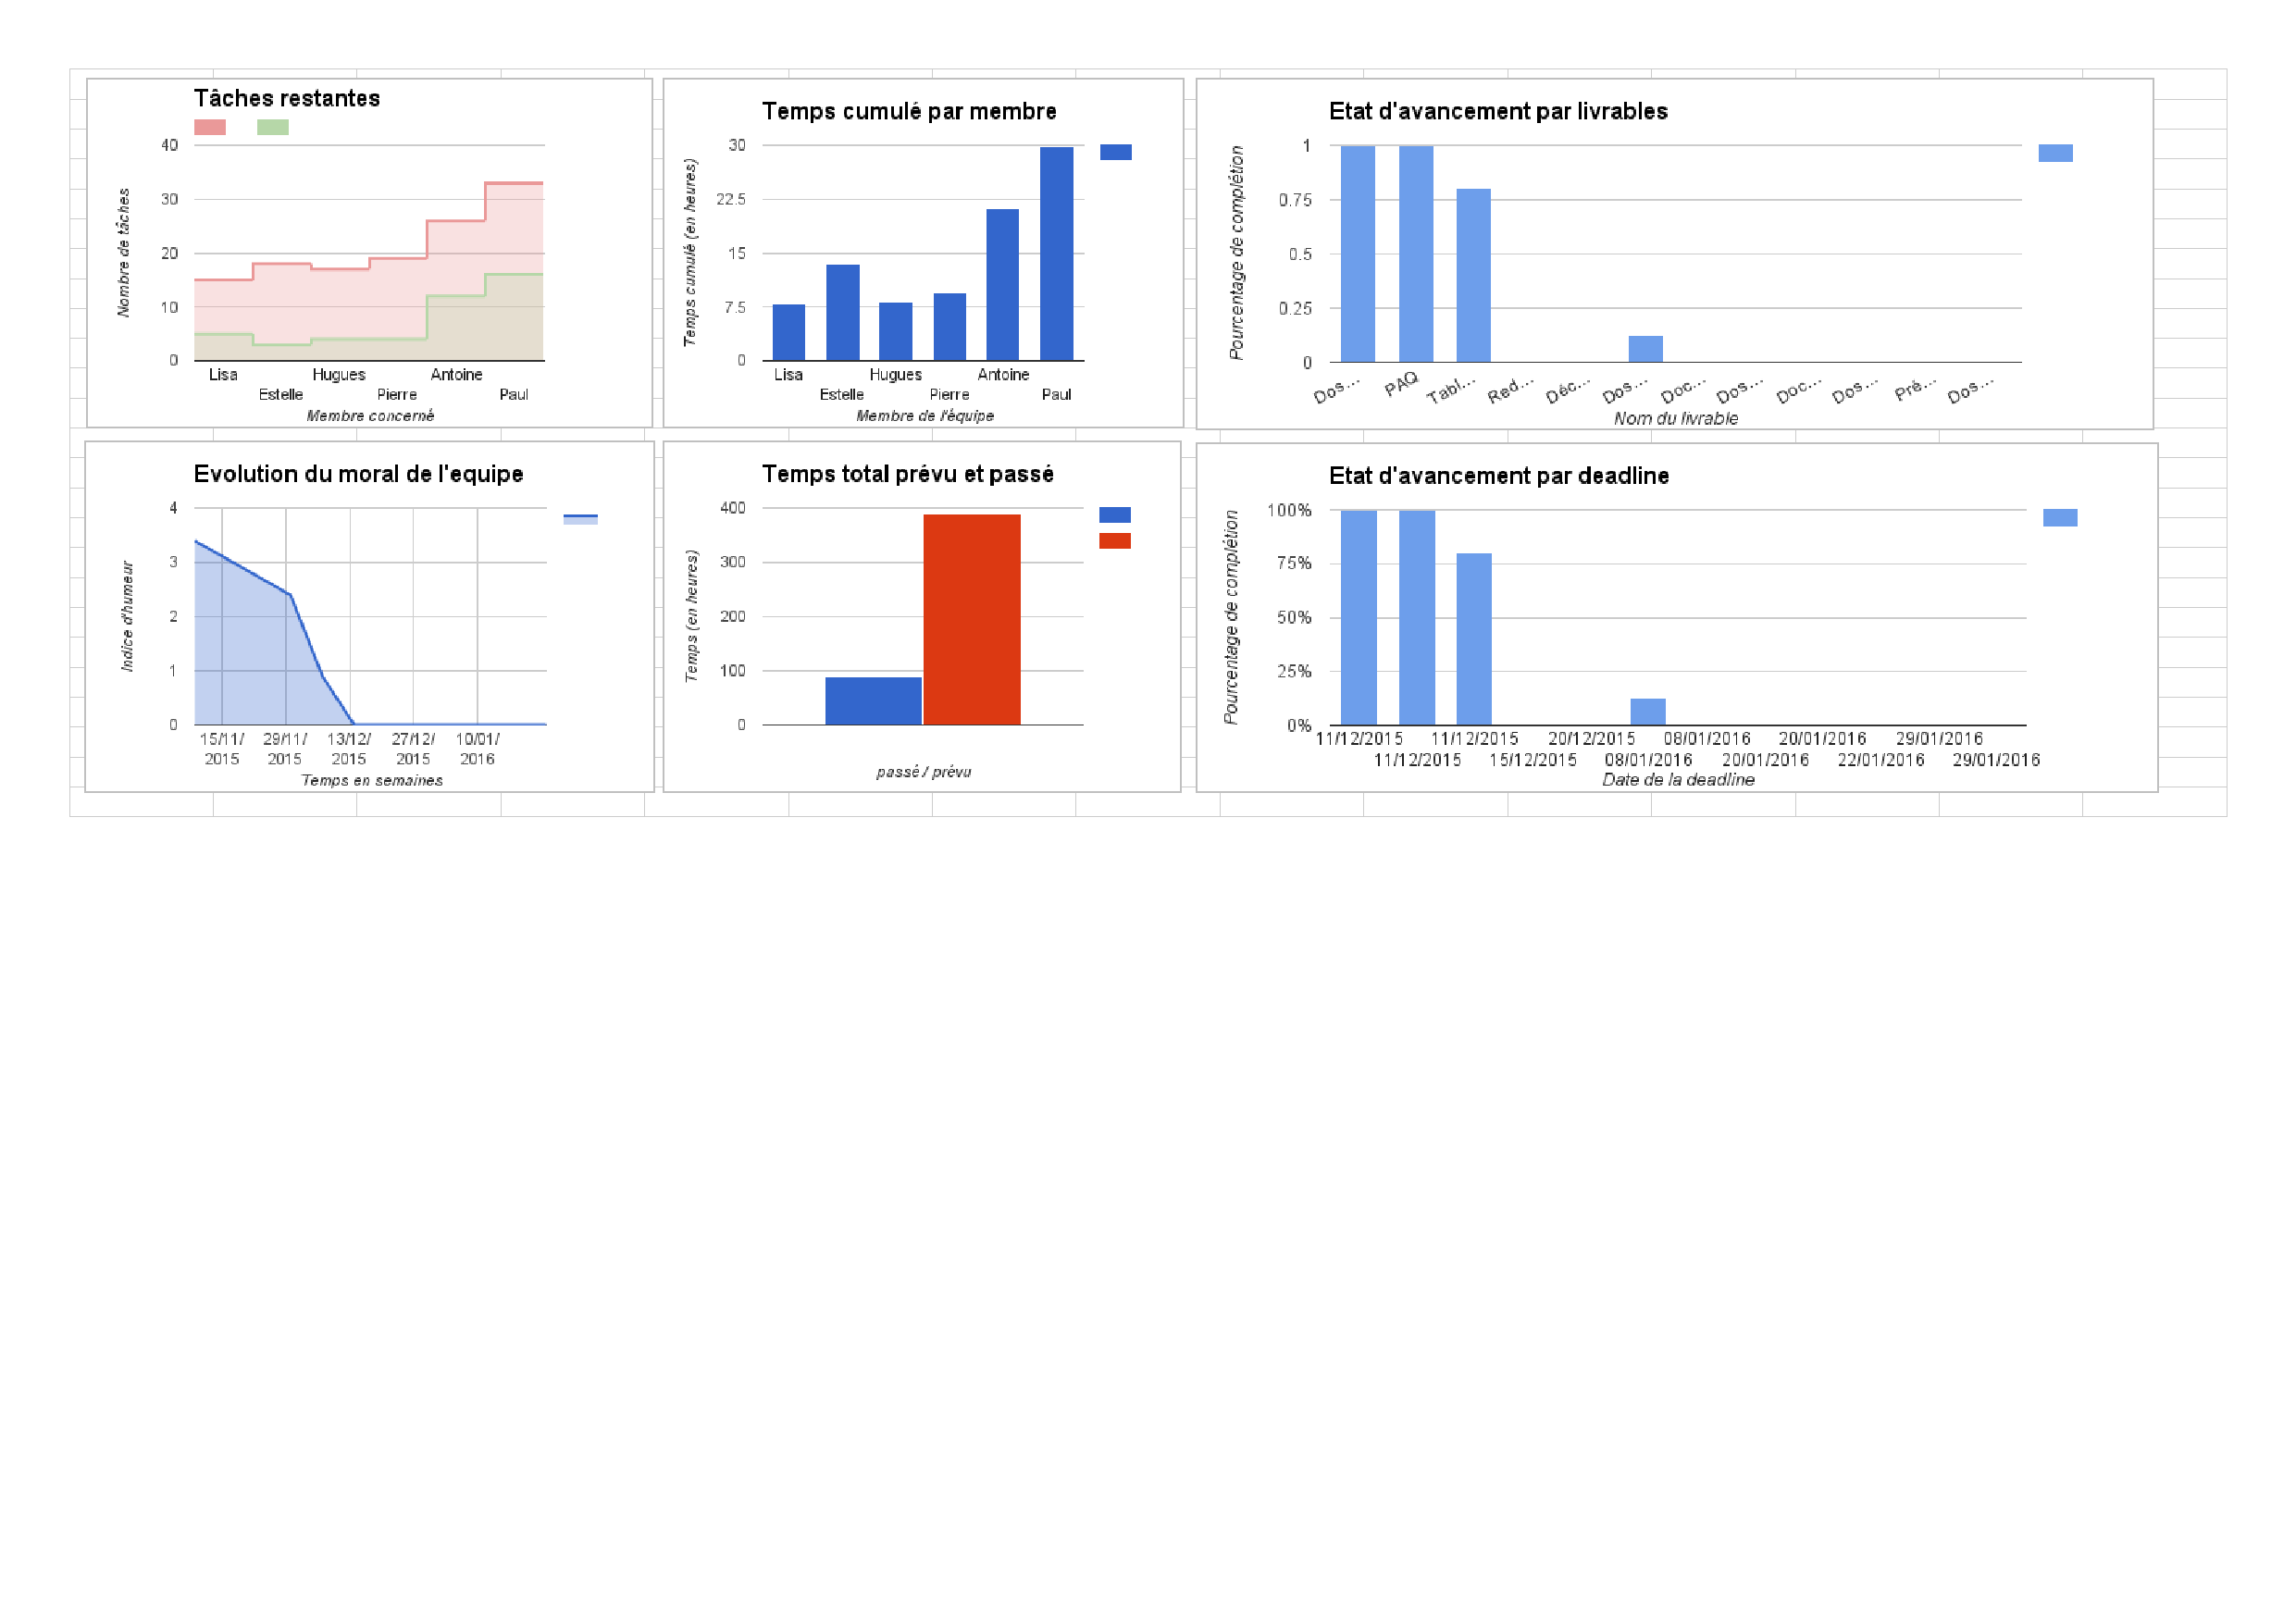
\includepdf[pages=-]{tdbs/Tableau_de_Bord_13-12-15.pdf}

\chapter{Tableau de Bord le 18/12/2015}
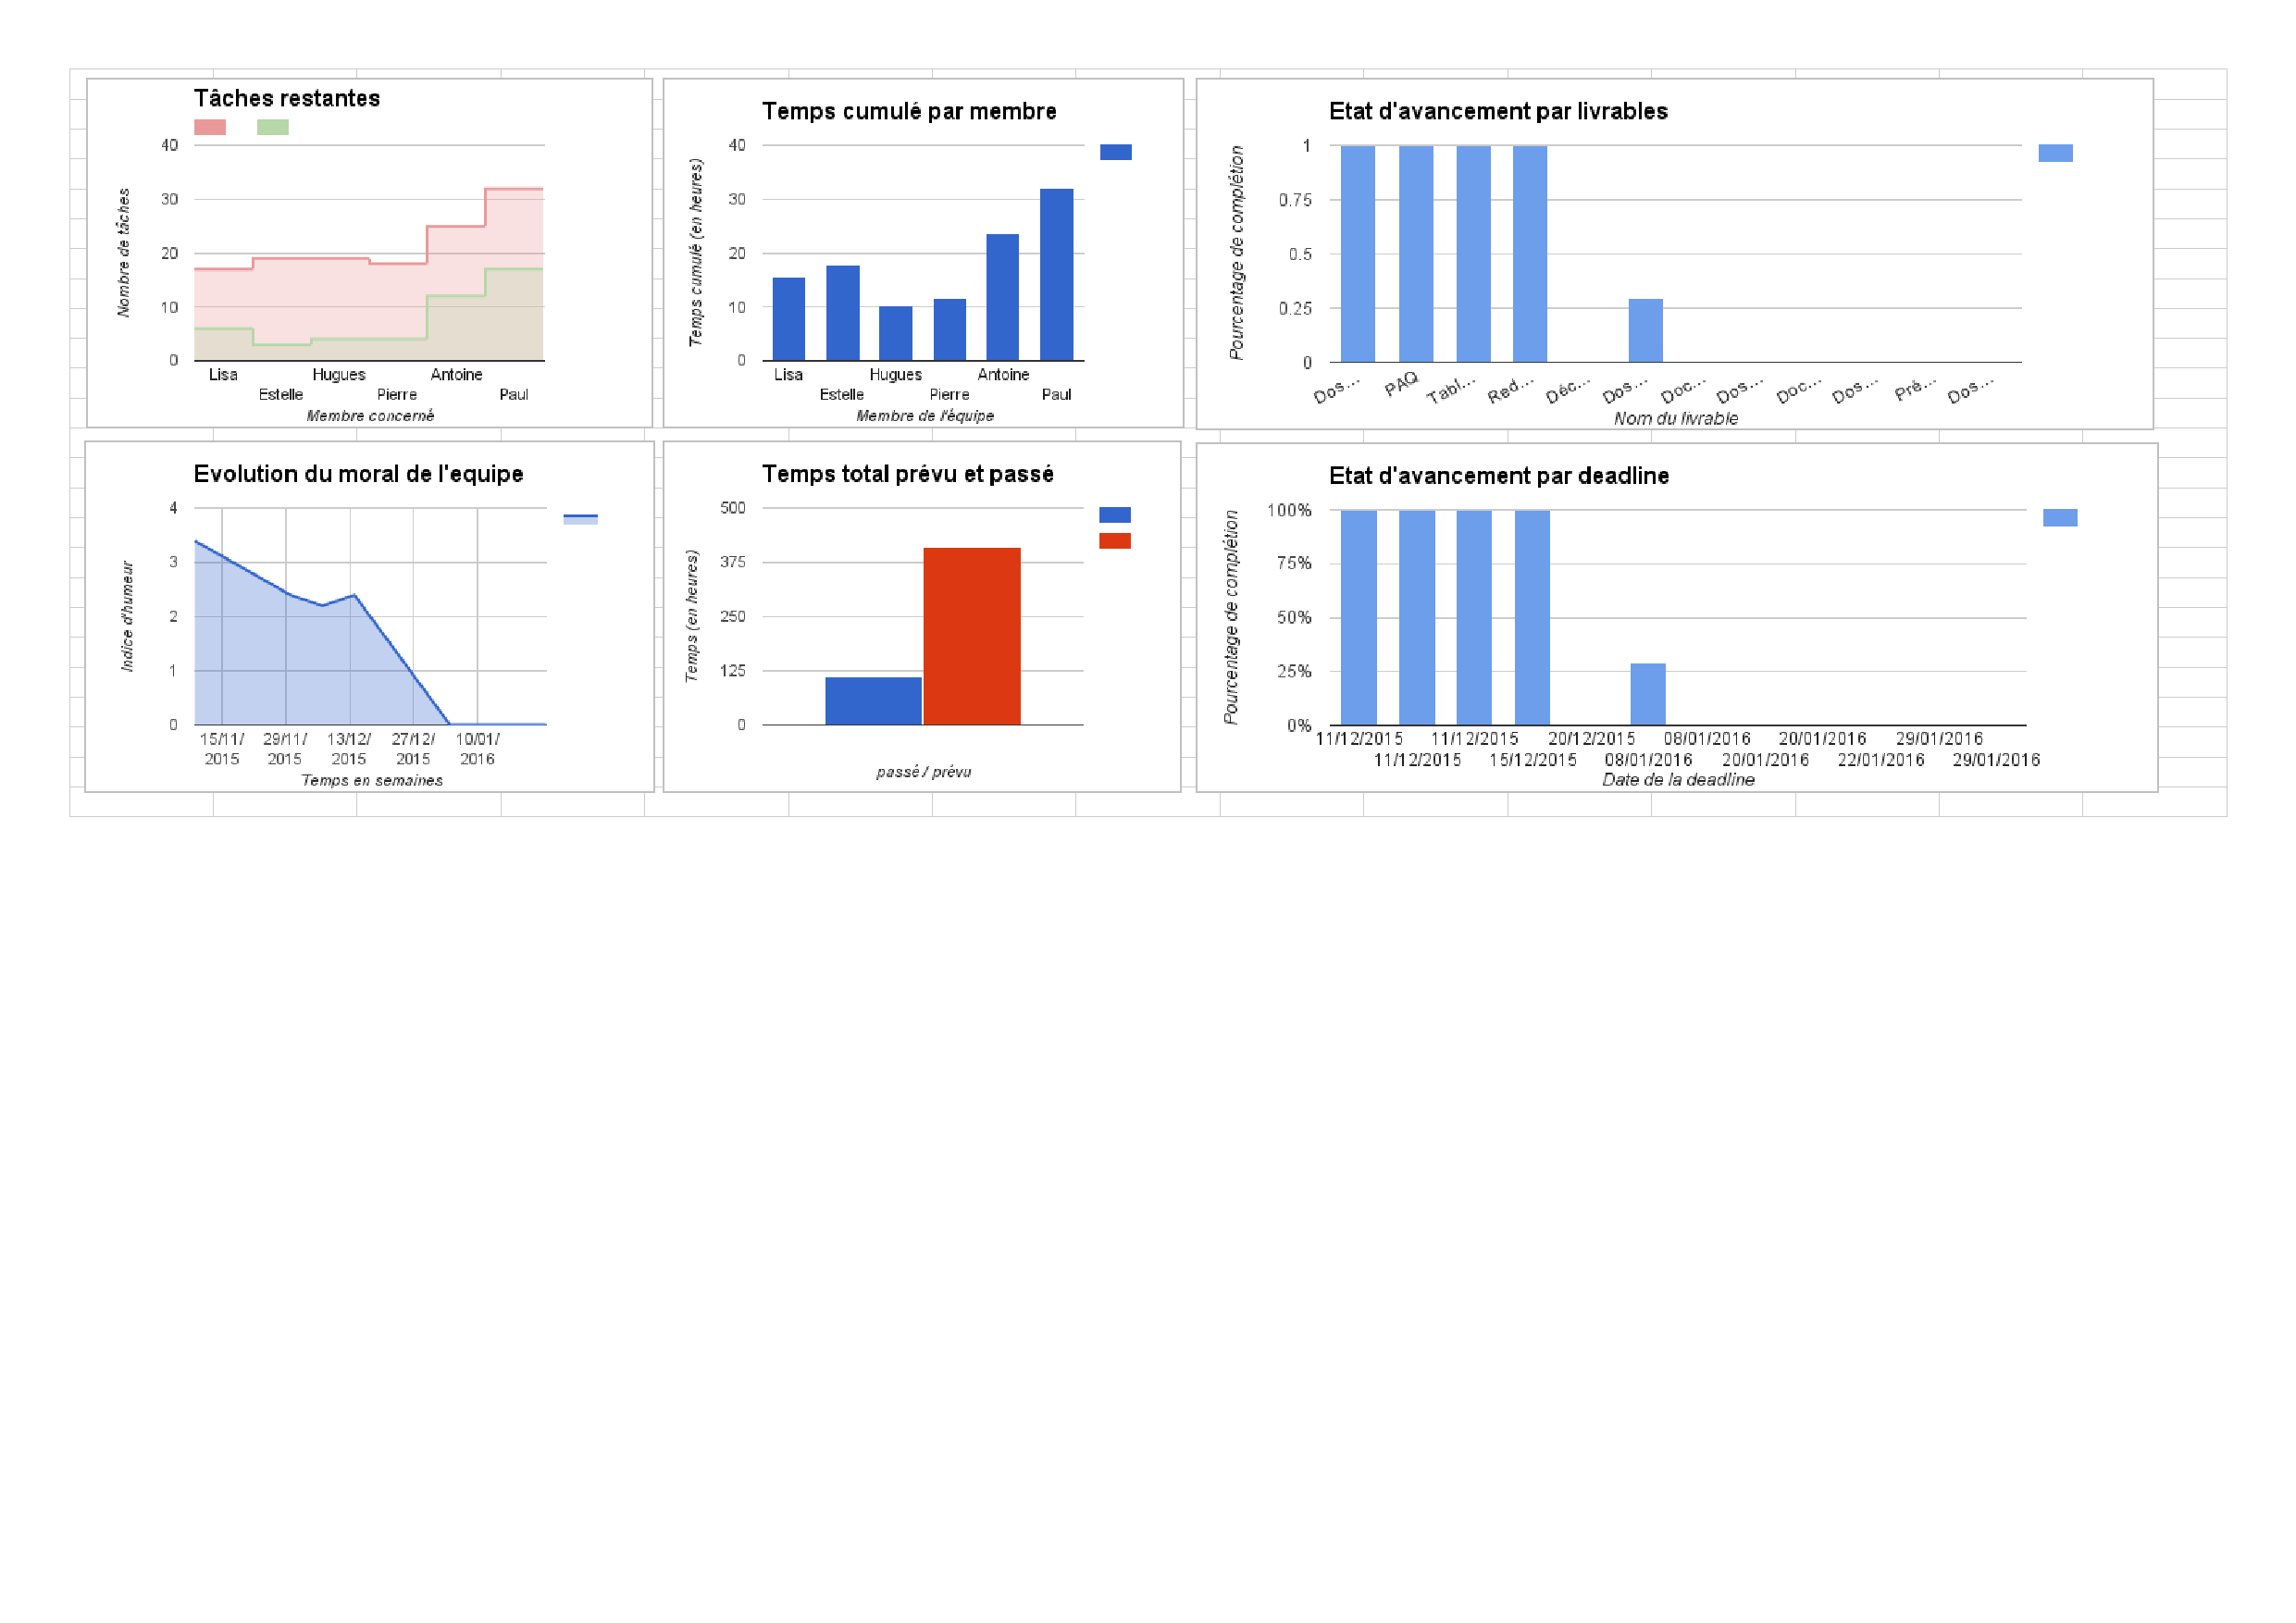
\includepdf[pages=-]{tdbs/Tableau_de_Bord_18-12-15.pdf}

\end{appendices}

%%% End document
\end{document}
